\lhead{\textbf{Basic Algorithms, Fall 2025 \\ CSCI-UA.0310-005/6}}
\chead{\Large{\textbf{Homework 12}}}
%%%%%%%%%%%%%%%%%%%%%%%%%%%%%%%%%%%%%%%
% ENTER NAME BELOW!
%%%%%%%%%%%%%%%%%%%%%%%%%%%%%%%%%%%%%%%
\rhead{\textbf{Professor Rachit Garg}\\\textbf{Name:} ~~~~~~~~~~~~~~~~~~~~~~~~~~~~~~~~~~~~~}
%REPLACE THE TILDES WITH YOUR NAME
\runningheadrule
\firstpageheadrule
\cfoot{}

\section*{Due December 8 (11:59 p.m.)}
\intro
\subsection*{0 List all your collaborators and sources: (\texorpdfstring{$-\infty$}{-∞} points if left blank)}
\vspace{0.75cm}

\section*{Problem 12-1 : Kruskal's and Prim's Algorithms (40 Points)}
\begin{figure}[h]
    \centering
    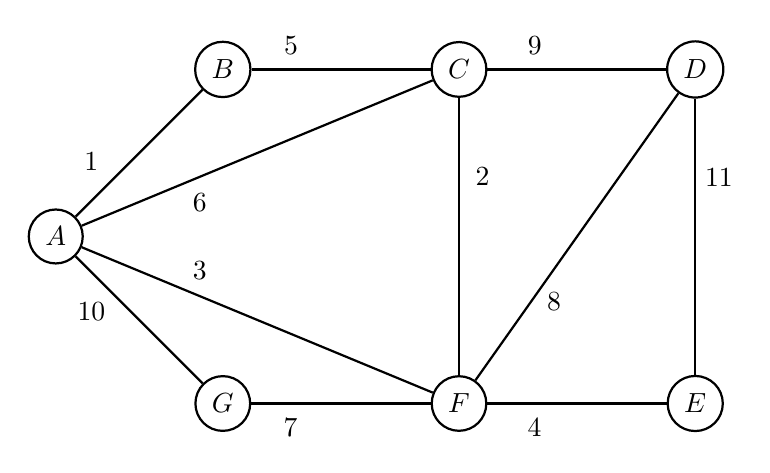
\begin{tikzpicture}[node distance={30mm}, thick,main/.style={circle, thick,draw,font=\sffamily\bfseries}, ar/.style={-{Stealth[scale=1.2]}}]
      \node[main] (1) {$A$}; 
      \node[main] (2) [above right of=1]{$B$};
      \node[main] (3) [right of=2]{$C$};
      \node[main] (4) [right of=3]{$D$};
      \node[main] (5) [below right of=1]{$G$};
      \node[main] (6) [right of=5]{$F$};
      \node[main] (7) [right of=6]{$E$};
      
      \draw (1) -- (2) node [at start, xshift=0.2cm, yshift=0.7cm]{$1$};
      \draw (1) -- (3) node [at start, xshift=1.5cm, yshift=0.3cm]{$6$};
      \draw (1) -- (5) node [at start, xshift=0.2cm, yshift=-0.7cm]{$10$};
      \draw (1) -- (6) node [at start, xshift=1.5cm, yshift=-0.3cm]{$3$};
      \draw (2) -- (3) node [at start, xshift=0.5cm, yshift=0.3cm]{$5$};
      \draw (3) -- (4) node [at start, xshift=0.6cm, yshift=0.3cm]{$9$};
      \draw (3) -- (6) node [at start, xshift=0.3cm, yshift=-1.0cm]{$2$};
      \draw (4) -- (7) node [at start, xshift=0.3cm, yshift=-1.0cm]{$11$};
      \draw (5) -- (6) node [at start, xshift=0.5cm, yshift=-0.3cm]{$7$};
      \draw (6) -- (7) node [at start, xshift=0.6cm, yshift=-0.3cm]{$4$};
      \draw (6) -- (4) node [at start, xshift=1.0cm, yshift=1.0cm]{$8$};
    \end{tikzpicture}
    \caption{\textbf{Undirected graph $\mathbf{G}$.}}
    \label{fig:mst}
\end{figure}

Consider the undirected weighted graph $G = (V, E)$ in Figure~\ref{fig:mst} above.
\newpage
\begin{enumerate}
    \item  (20 points) Run Kruskal's algorithm on this graph, and record the edge that is \emph{added to the tree} at each step.
        We have filled the first step in for you.
        (Note: write only the edge that is added to the tree at each step, not every edge that is considered.)

    \begin{solution}
    %\vspace{1cm}
    \begin{center}
    \begin{tabular}{c|c|c|c|c|c|c|c}
         \textbf{Step} & 1 & 2 & 3 & 4 & 5 & 6\\
         \hline
     \textbf{Edge Added} & $\left\{A, B \right\}$ & \hspace{1cm}   &   \hspace{1cm} &   \hspace{1cm} &   \hspace{1cm} & \hspace{1cm}  \\
    \end{tabular}
    \end{center}
    \end{solution}
    
    \item (20 points) Now do the same for Prim's algorithm, starting from vertex $A$.

    \begin{solution}
    %\vspace{1cm}
    \begin{center}
    \begin{tabular}{c|c|c|c|c|c|c|c}
         %\textbf{Step} & 1 & 2 & 3 & 4 & 5 & 6\\
         %\hline
         %\textbf{Edge Added} & $AB$ &   &   &   &   &  \\
         \textbf{Step} & 1 & 2 & 3 & 4 & 5 & 6\\
         \hline
     \textbf{Edge Added} & $\left\{A, B \right\}$ & \hspace{1cm}   &   \hspace{1cm} &   \hspace{1cm} &   \hspace{1cm} & \hspace{1cm}  \\
    \end{tabular}
    \end{center}
    \end{solution}
    
\end{enumerate}

\section*{Problem 12-2 (20 Points)}

Let $G = (V,E)$ be an undirected, connected graph, with non-negative edge weights $w : E \rightarrow \mathbb{R}^{\geq 0}$.
Although in general multiple edges can have the same weight,
for this problem we assume that there is a unique lightest edge $e_{\min}$ and a unique heaviest edge $e_{\max}$ in the graph.
The other edges can have non-unique weights, but no edge except $e_{\min}$ has weight $w(e_{\min})$,
and similarly for $e_{\max}$.

\begin{enumerate}
    \item (10 points) 
        Is it true that \emph{every} MST of $G$ must contain the lighest edge $e_{\min}$? If true, explain why. If not, show a counter-example.
    \begin{solution}
        \vspace{5cm}
    \end{solution}
    \newpage
    \item (10 points)
        Is it true that \emph{no} MST of $G$ can contain the heaviest edge $e_{\max}$? If true, explain why. If not, show a counter-example.
    \begin{solution}
        \vspace{5cm}
    \end{solution}
    %\item (Honors problem, ***, 0 points) Prim's algorithm and Kruskal's algorithm may not always give the same MST
        %when we run them on the same weighted graph.
        %In fact, there can even be different executions of Prim that return different MSTs, and similarly for Kruskal (as we saw in class).
        %Give a \emph{necessary and sufficient condition} on a weighted graph,
        %such that this condition holds if and only if
        %any execution of Prim
        %and any execution of Kruskal on the graph return the same MST.
        %%For this problem, assume Prim's algorithm chooses a starting node arbitrarily. Give a necessary and sufficient condition on $G$ for when Prim's and Kruskal's will always return the same MST of $G$. 
    %\begin{solution}
        %\vspace{7cm}
    %\end{solution}
\end{enumerate}

\section*{Problem 12--3 Cuts and Components (15 Points)}

Let $C_1, C_2 \subseteq V$ be two disjoint sets of vertices in an undirected connected graph $G = (V,E)$,
and let $w : E \rightarrow \mathbb{R}^{\geq 0}$ be a weight function on the edges.
Let $e$ be a lightest edge among all the edges that have one endpoint in $C_1$ and the other in $C_2$;
that is, $e = \left\{ u, v \right\}$ is an edge such that $u \in C_1, v \in C_2$, and
\begin{equation*}
    w(e) = \min_{ e' = \left\{x,y\right\} : x \in C_1, y \in C_2 } w(e').
\end{equation*}

\medskip
\noindent\textbf{True or false:} There must exist an MST of $G$ that contains $e$.

\noindent If true, explain why, and if false, show a counter-example.

\medskip
\noindent Note: unlike the "light-is-safe" theorem from class, here the sets $C_1$ and $C_2$
do \emph{not} need to cover all vertices of the graph.
In other words, it could be that $C_1 \cup C_2 \neq V$.

    \begin{solution}
        \vspace{8cm}
    \end{solution}

\section*{Problem 12-4 : MST Reduction (25 Points)}
Suppose you are given an algorithm $P$ that can solve the MST problem on undirected graphs with \emph{non-negative} edge weights,
and the running time of $P$ on graphs with $n$ vertices is $T(n)$.
However, $P$ cannot solve MST on graphs with \emph{negative} weights, and in fact we do not know what will happen if we try to run $P$ on such a graph; the computer may catch on fire.

Design an algorithm $P'$ that \emph{uses $P$},
and solves the MST problem on undirected graphs where the edges weights are allowed to be negative.
Your algorithm can \emph{call $P$} as a subroutine, but you can only give $P$ as input a graph that has non-negative weights.
The runtime of $P'$ (including any calls it makes to $P$) should be $O(|V| + |E| + T(|V|) )$.

\begin{enumerate}
    \item (15 points) Describe your algorithm $P'$, and explain why it is correct.
    \begin{solution}
        \vspace{8cm}
    \end{solution}
    \item (10 points) Explain the runtime of your algorithm. 
    \begin{solution}
        \vspace{5cm}
    \end{solution}
\end{enumerate}

